{
{\sffamily Dette afsnit har til formål at beskrive hvordan vi trækker
regioner ud af billedet. Kort sagt forsøger vi at segmentere billedet
ved primært ved at bruge en metode kaldet floodfill. Billedet bliver
først præpareret ved at finde kanter, en metode betegnet som
kantdetektion, og viske farverne sammen ved en metode kaldet sløring. Vi
vil i det følgende forklare, hvordan vi kombinerer disse metoder til at
finde regioner i en digital gengivelse af et maleri. Vi vil også komme
ind på hvilke andre metoder vi har forsøgt os med.
%navnligt den funktion i OpenCV der er buggy, GoodFeaturesToTrack og
%Perona and Malik fra Octave. Det følgende afsnit om Floodfill bør være
%en del af dette afsnit, ligesom vi skal have lignende beskrivelser af
%sløring og kant detektion.
}

\subsection{Floodfill\label{subsec_floodfill}}                                  % Denne metode er udgangs punktet
% Denne fil er inkluderet i udtraekning_af_regioner.tex
{

Floodfill finder de områder i et billede, hvis farve ligger inden for en
vis afvigelse af den originale farve. Der vælges en pixel i billedet,
som har en farve angivet ved en RGB-værdi. Ud fra denne pixel findes de
fire tilstødende pixels i lodret og vandret bane, som vist i figur
\ref{floodfill1}.

\begin{figure}[!h]
    \begin{center}
        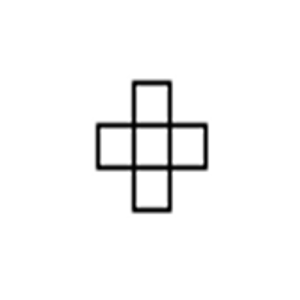
\includegraphics[scale=0.42,angle=0]{afsnit/vores_implementation/billeder/flood_fill/floodfill1}
    \end{center}
    \caption[]{Måden hvorpå floodfill arbejder med pixels i billedet.}
    \label{floodfill1}
\end{figure}

\subsubsection{Metode}
De følgende 3 skridt beskriver, hvordan floodfillmetoden virker i et
billede.

\begin{enumerate}
    \item Algoritmen starter med at markere den midterste pixel (vores
        startpixel) med et rødt flag, som angiver, at denne pixel bliver
        farvet. Nabopixels får et blåt flag, som angiver, at de skal
        kontrolleres for, om deres farve er inden for afvigelsen. Blå
        flag sættes kun, hvis en pixel ikke har noget flag i forvejen.
        Se figur \ref{floodfill2}.
    \item Hver pixel med et blåt flag kontrolleres for, om deres farve
        ligger indenfor afvigelsen. Hvis farven er inden for afvigelsen,
        bliver denne pixel sat i en liste og markeret med et grønt flag
        og et tal. Se figur \ref{floodfill3}.
    \item En pixel med grønt flag tages ud af listen og bliver sat til
        den nye startpixel. Skridt $1$ og $2$ bliver gentaget, til der
        ikke er flere grønne flag. Se figur \ref{floodfill4}.
\end{enumerate}

\begin{figure}[!h]
    \begin{center}
        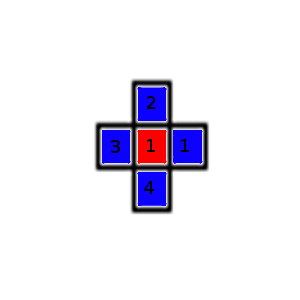
\includegraphics[scale=0.42,angle=0]{afsnit/vores_implementation/billeder/flood_fill/floodfill2}
    \end{center}
    \caption[]{Pixels efter første skridt i algoritmen. Den røde pixel
    er vores startpixel. Pixels, markeret med blåt, skal kontrolleres for
    deres farve. Numrene angiver rækkefølgen hvori de bliver gennemgået.}
    \label{floodfill2}
\end{figure}

\begin{figure}[!h]
    \begin{center}
        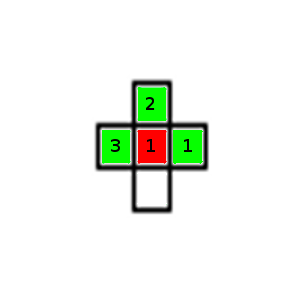
\includegraphics[scale=0.42,angle=0]{afsnit/vores_implementation/billeder/flood_fill/floodfill3}
    \end{center}
    \caption[]{Pixels efter andet skridt i algoritmen. De pixels, som har
    en farve, der ligger inden for afvigelsen, bliver markeret med et grønt
    flag og tildelt et tal, som angiver rækkefølgen. I denne illustration
    er den nederste pixel ikke blevet farvet grøn. Den var før blå, men
    da den ikke ligger inden for afvigelsen, mister den sit flag.}
    \label{floodfill3}
\end{figure}

\begin{figure}[!h]
    \begin{center}
        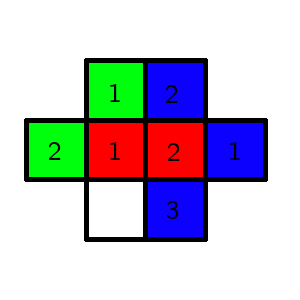
\includegraphics[scale=0.42,angle=0]{afsnit/vores_implementation/billeder/flood_fill/floodfill4}
    \end{center}
    \caption[]{Pixels efter skridt tre og et nyt skridt 1. Vi har valgt
    den grønne pixel, med det laveste tal, fra figur \ref{floodfill3} som
    ny startpixel. Nye pixels markeret med blåt mangler at blive
    kontrolleret.}
    \label{floodfill4}
\end{figure}

På denne måde itererer metoden sig igennem alle de pixels, som ligger
inden for en vis afvigelse fra startfarven. Metoden kan bruges på to
måder; enten kan man regne varianten fra den første startpixel ud, og
således kun have én startfarve, eller man kan ændre den efter den nye
startpixel --- som bliver fundet i tredje skridt --- og således have en
startfarve, der ændres efterhånden. Det skal bemærkes, at den pixel, som
i figur \ref{floodfill3} mister sit blå flag, godt kan blive taget i
betragtning igen senere, når vi vælger en ny startpixel. En pixel kan
dog højst blive taget i betragtning i alt fire gange, fordi den har fire
tilstødende pixels.

\subsubsection{Eksempler}
Vi vil nu eksemplificere, hvordan denne metode virker i praksis ved
manipulation af billedet vist i figur \ref{bathers}.  Dette billede er
valgt, da det har været brugt i flere argumenter for, at man i
malerkunsten finder særligt mange interessante regioner i det gyldne
snit\cite{GoldenNumber,RatioArt}. Endvidere er maleriet
interessant at teste på, da det er udført i det, der kaldes
pointilistisk stil, hvilket vil sige, at maleriet faktisk består af en
masse små prikker. I de fem billeder vist i figur
\ref{dot_ff_fixed_7_7}, \ref{dot_ff_var_7_7}, \ref{dot_ff_fixed_10_10},
\ref{dot_ff_var_10_10} og \ref{dot_ff_var_9_9} bruges floodfill på den
pixel, der er at finde i midten af den røde prik. Den tilladte afvigelse
gives som parret $(lo, up)$ med en værdi for, hvor meget RGB-værdien må
henholdsvis falde og stige. Det anbefales at studere figurene og den
tilhørende tekst.

% Det her billede opfører sig underligt mht. scale :/
\begin{figure}[!h]
    \begin{center}
        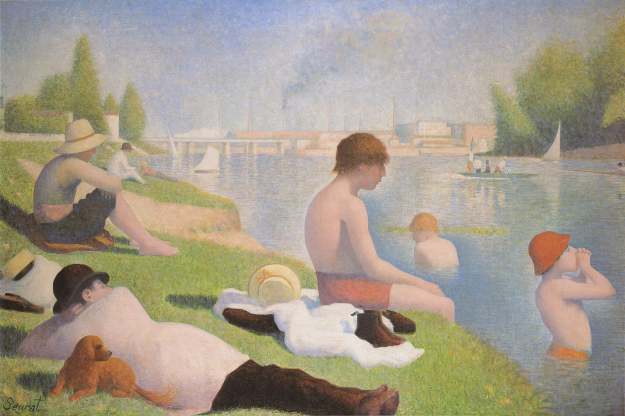
\includegraphics[scale=8]{afsnit/vores_implementation/billeder/flood_fill/seurat_bathers}
    \end{center}
    \caption[George Seurat: \emph{Bathers at Asnieres} -- 1884]{George
    Seurat: \emph{Bathers at Asnieres} - 1884\\Originalt billede.}
    \label{bathers}
\end{figure}

\begin{figure}[!h]
    \begin{center}
        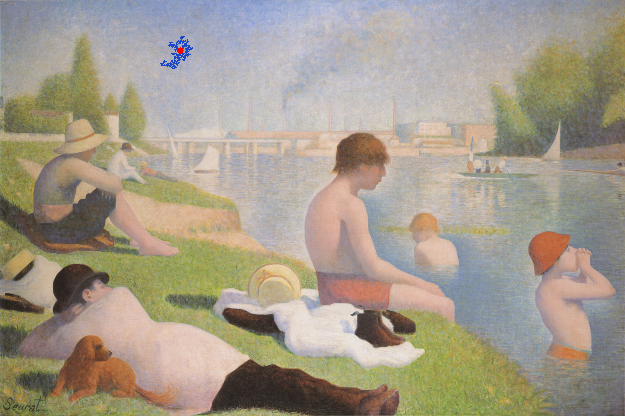
\includegraphics[scale=0.49]{afsnit/vores_implementation/billeder/flood_fill/dot_ff_fixed_7_7}
    \end{center}
    \caption[]{Floodfill-metoden i et billede, hvor der kun sammenlignes
    med farven på den originale pixel med afvigelsen $(7,7)$.}
    \label{dot_ff_fixed_7_7}
\end{figure}

\begin{figure}[!h]
    \begin{center}
        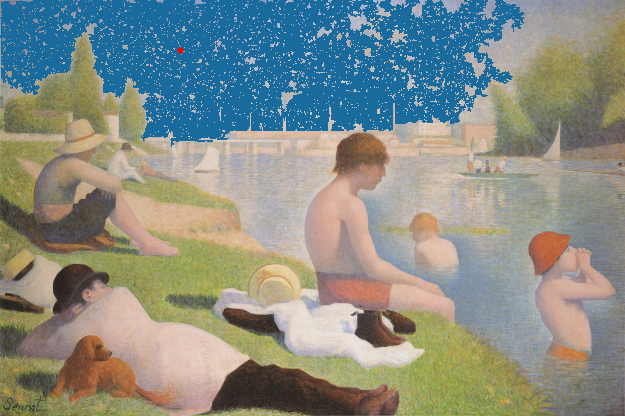
\includegraphics[scale=0.49]{afsnit/vores_implementation/billeder/flood_fill/dot_ff_var_7_7}
    \end{center}
    \caption[]{Floodfill-metoden i et billede, hvor der sammenlignes med
    farven på den nye startpixel. Afvigelsen er sat til $(7,7)$ ligesom
    i figur \ref{dot_ff_fixed_7_7}. Det ses, at vi nu dækker et meget
    større areal.}
    \label{dot_ff_var_7_7}
\end{figure}

\begin{figure}[!h]
    \begin{center}
        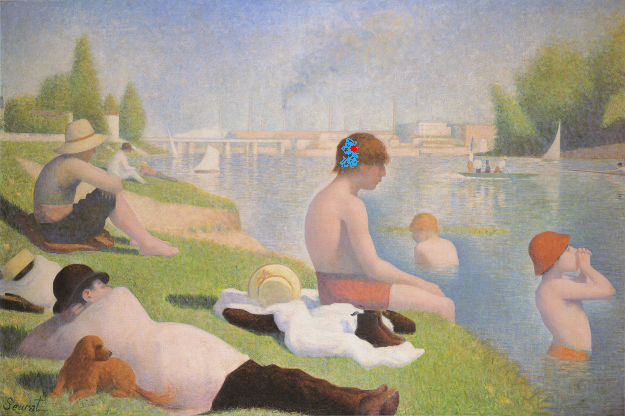
\includegraphics[scale=0.49]{afsnit/vores_implementation/billeder/flood_fill/dot_ff_fixed_10_10}
    \end{center}
    \caption[]{Floodfill-metoden i et billede, med udgangspunkt i en ny
    pixel, hvor der kun sammenlignes med den originale pixel. Den
    tilladte afvigelse er på $(10,10)$.}
    \label{dot_ff_fixed_10_10}
\end{figure}

\begin{figure}[!h]
    \begin{center}
        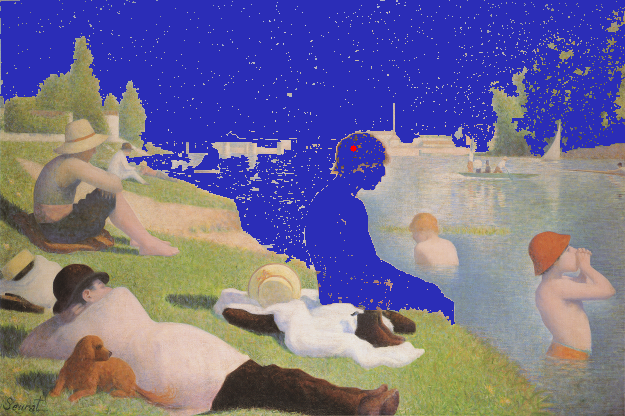
\includegraphics[scale=0.49]{afsnit/vores_implementation/billeder/flood_fill/dot_ff_var_10_10}
    \end{center}
    \caption[]{Floodfill med samme udgangspunkt og afvigelse som i figur
    \ref{dot_ff_fixed_10_10}, men der sammenlignes nu med den nye
    startpixel. Med en større tilladt afvigelse, breder floodfill sig
    meget mere og smelter både himmel, hav og dreng sammen.}
    \label{dot_ff_var_10_10}
\end{figure}

\begin{figure}[!h]
    \begin{center}
        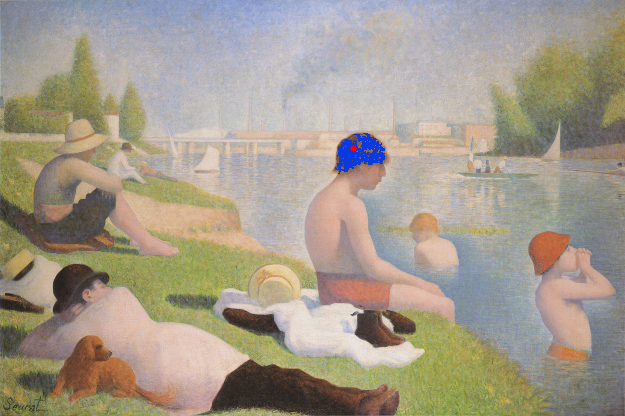
\includegraphics[scale=0.49]{afsnit/vores_implementation/billeder/flood_fill/dot_ff_var_9_9}
    \end{center}
    \caption[]{Floodfill med samme udgangspunkt som i figur
    \ref{dot_ff_fixed_10_10} og \ref{dot_ff_var_10_10}. Her bruges igen
    sammenligning med ny startpixel, men nu med en afvigelse på $9,9$.
    Denne lille ændring er nok til, at vi holder os pænt indenfor den
    region som udgøres af drengens hår.}
    \label{dot_ff_var_9_9}
\end{figure}

\subsubsection{Hvilken metode passer bedst?}
Som nævnt ovenfor, og illustreret i billederne, er der to måder vi kan
bruge floodfill på. Hvis man vælger at regne varianten ud fra den første
startpixel, ses det, at metoden vil indskrænke sig meget og ikke komme
ind i alle hjørner af en region. Til gengæld har denne fremgangsmåde
sværere ved at krydse kanter og på den måde komme ind i en ny region.

Vælger man at ændre varianten efter den nye startpixel, ses det, at man
vil male større regioner. Da denne fremgangsmåde hele tiden tilpasser
varianten, kan man medtage regioner, der langsomt skifter farve. Et godt
eksempel ses i figur \ref{dot_ff_var_10_10}, hvor drengens krop og
bukser bliver set som sammenhængende. Dette er interessant, især med
hensyn til digitale billeder af malerier, da solen eller blitzens
refleksion kan påvirke billedets farver. Af samme grund er den
fremgangsmåde heller ikke særlig følsom over for kanter, hvilket
resulterer i, at man let kommer til at gå ind i andre regioner.

Vi har valgt at benytte os af den sidstnævnte metode, da den efter vores
mening giver det bedste resultat. Vi vurderer, at det er vigtigere at
tage højde for sol og små farveskift end at være sikker på, at vi ikke
går ud over kanterne. Vi vil senere beskrive, hvordan vi på anden vis
sikrer, at vi beholder kanterne.

Som illustreret i billederne skal vi dog stadig tage højde for, hvordan
vi vil sætte tærskelværdierne. Indtil videre bliver de sat efter, hvad
der giver det mest illustrative resultat.

%For at få denne metode til at virke på 25000 billeder, hvor en del af
%billederne ikke har samme farvetone eller er blevet falmet, må der
%for hvert billede udregnes hvad for en varians i farve der skal bruges.

}

% vim: set tw=72 spell spelllang=da:


\subsection{Sløring}                                    % Her maler vi større regioner
% Denne fil er inkluderet i udtraekning_af_regioner.tex
{
Sløring, som kommer fra det engelske ord ``blur'', er en gruppering af
filtre som bruges til at fjerne støj og uregelmæssigheder i billeder. Vi
så i afsnit \ref{subsec_floodfill}, at metoden floodfill nogle gange kan
have svært ved at fylde hele regionen ud. Specielt i figur
\ref{dot_ff_var_7_7} ses at himlen har små huller. En sløring af
billedet kan hjælpe med at glatte farverne ud, således at vi dækker mere
af regionen. Sløring af billedet kan også hjælpe til at fjerne diverse
artefakter, såsom revner eller pletter i billedet. Specielt i
vores testbillede, der som tidligere nævnt er malet med en masse
prikker, er det en stor hjælp at sløre billedet, så farverne bliver mere
ensartede. Vi vil nu se på tre forskellige måder at opnå dette på.

De to første metoder har svært ved at bibeholde kanterne i et billede,
men arbejder til gengæld direkte på billedet. Den tredie metode
bibeholder til en vis grad kanterne bedre, men kan ikke arbejde direkte
på billedet, hvilket kræver et større pladsforbrug. Metoden som bruges
til de 2 første sløringer, heder foldning, som bruger en kernel til
udregning af ny farver. En kernel er en lille matrice, som betegner hvor
stor del af billedet og hvor meget af pixels værdiger fra farverne rund
om et punkt, skal tages med i udregningen for den nye sløret farve. En
kernel kan ses i figur \ref{Foldning}. Foldning er en simpel matematisk
metode, som beskriver hvordan man kan gange 2 matricer sammen, i vores
tilfælde, en kernel $\mathbb{Z}^{n}\times{} \mathbb{Z}^{m}$ og et
billedet matrice $\mathbb{Z}^{k}\times{} \mathbb{Z}^{d}$, hvor $n = d
~\vee~ m = k$ ikke behøver at være opfyldt.

\begin{figure}[h]
	\begin{center}
		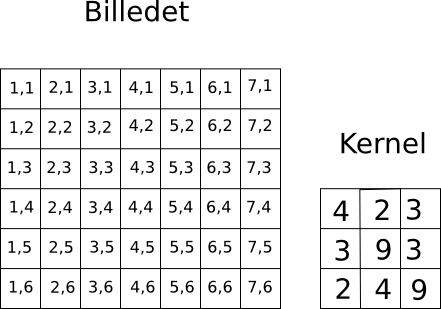
\includegraphics[scale=1,angle=0]{afsnit/vores_implementation/billeder/sloering/convolution}
	\end{center}
	\caption[]{Et billedet hvor x,x betegner plaseringen og en kernel med 9 tilfældige tal fra 0 til 9}
	\label{Foldning}
\end{figure}

Som man kan se i figur \ref{Foldning} er selve billedet og kernel i
vid forskellige størrelser. Måden Foldning virker på, er at man
multiplicere kernelen ovenpå de værdiger som ligger rund om den pixel,
som vi gerne vil finde den sløret farve af og tager gennemsnittet af den
værdig, f.eks farven på pixel $(4,4)$, bliver

\begin{equation}
	(4,4) = ((3,3)*4+(4,3)*2+(5,3)*3+(3,4)*3+(4,4)*9+(5,4)*3+(3,5)*2+(4,5)*4+(5,5)*9)*\frac{1}{39} 
\end{equation}

I dette eksempel, er punktet $(5,5)$ og $(4,4)$ vægtet højre i forhold
til de andet, så farven vil blive sløret i den retning. Dette skyldes at
kernelen er bygget tilfældig op, i en rigtige sløring er kernelen meget
specifikt udvalgt for at give det beste resultat.

\subsubsection*{Simpel sløring}
I metoden simpel sløring er der 3 steps, først udregnes en kernel. Multiplicere
kernel rigtigt på billedet, kaldet Foldning. Sættes værdigerne fra
multiplikationen ind i billedet, som så bliver det nye sløret billedet nå
alle punkter er omdannet. kernel for den simple sløring er en kvadradisk
matrice med kun talet 1 i. Resultatet for en simpel sløring kan ses i
figur \ref{simple_metode}

\subsubsection*{Gaussisk sløring}
Gaussisk sløring har de samme 3 steps som simpel sløring. 
Måde Gaussisk sløring udregner sin kernel, at ved brug af Normale
fordeling, som betegnet med denne formel

\begin{equation}
	G(x,y) = \frac{1}{2\pi\sigma^2}e^{-\frac{x^2+y^2}{2\sigma^2}}
\end{equation}

Vi sætter $\sigma = 1$ og lader x og y bevæge sig fra -1 til 1, med skridt størrelse
på 1. Den upscalet afrundet kerne kan se på figur \ref{gauss}.

\begin{figure}[h]
	\begin{center}
		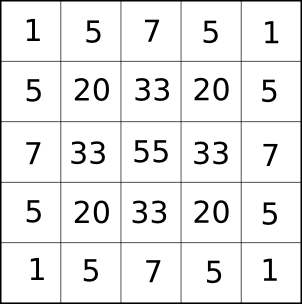
\includegraphics[scale=0.5,angle=0]{afsnit/vores_implementation/billeder/sloering/gauss}
	\end{center}
	\caption[]{En $3~\times{}~3$ Kernel for gauss sløring}
	\label{gauss}
\end{figure}

Denne kernel kan så bruges ved hjælp af foldning til at danne det sløret
billet, som vi kan se i figur \ref{gaussian_metode}

\subsubsection*{Sløring ved statistisk median}
Den sidste metode vi vil nævne er i grunden meget simpel. Grundidéen er
at finde den statistiske median i pixelværdierne rundt om en givet pixel
og tildele medianværdien til denne. Givet et antal pixels, er det
trivielt at sætte dem i en liste og sortere dem efter deres værdi. Hvis
antallet af elementer i listen er ulige, er det midterste element i den
sorterede liste medianen. Er der et lige antal elementer i listen,
defineres medianen som gennemsnittet af de to midterste elementer.
Pixels vælges i et $N \times M$ vindue med den originale pixel i
centrum, som vist i figur \ref{red_box_nxm} og vi vil således altid have
et ulige antal elementer i listen.

\begin{figure}[!h]
    \centering
    \subfloat[]{\label{red_box_nxm}
        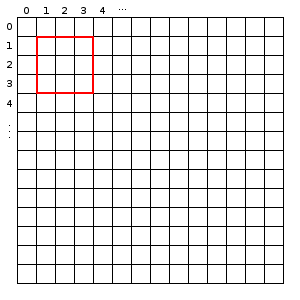
\includegraphics[scale=0.42,angle=0]{afsnit/vores_implementation/billeder/sloering/red_pixel_box}
    }\\
    \subfloat[]{\label{3_3_vindue}
        \renewcommand{\arraystretch}{1.8}
        \begin{tabular}{|c|c|c|}
            \hline
            35 & 98  & 23 \\\hline
            48 & \cellcolor[gray]{0.5}42 & 0 \\\hline
            8  & 12   & 29 \\\hline
        \end{tabular}
        }\hspace{1em}
    \subfloat[]{\label{sorteret_median}
        \renewcommand{\arraystretch}{1.5}
        \centering
        \begin{tabular}{|c|c|c|c|c|c|c|c|c|}
            \hline
            0 & 8 & 12 & 23 & \cellcolor[gray]{0.5}29 & 35 & 42 & 48 & 98\\\hline
        \end{tabular}
        }
        \caption[]{
            Bestemmelse af median for pixel med koordinaterne $(2, 2)$.
            \textbf{\ref{red_box_nxm})} Pixels i et $3\times3$ vindue
            omkring $(2, 2)$ er markeret med rødt.
            \textbf{\ref{3_3_vindue})} Værdierne i $3\times3$ vinduet.
            Det ses den originale pixel har værdien $42$.
            \textbf{\ref{sorteret_median})} Den sorterede liste med
            værdierne fra vinduet. Det ses at medianen har værdien
            $29$. Den originale pixel vil da skifte værdi fra $42$ til
            $29$.
        }
\end{figure}

Denne metode kan ikke køres direkte på det originale billede, da dette
vil interferere med fastsættelse af medianen for alle pixels. Man må
derfor oprette en kopi af det originale billede og sætte de fundne
medianværdier i denne. Man finder således altid medianen i forhold til det
originale billede.

\subsubsection*{Eksempler}

% Hold on, this is figure-madness
\begin{figure}[!h]
    \centering
    \subfloat[Original]{\label{simple_original}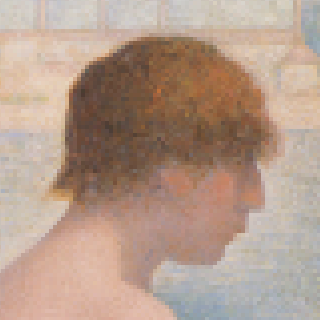
\includegraphics[angle=0,width=0.3\textwidth]{afsnit/vores_implementation/billeder/sloering/original}}\hspace{1em}
    \subfloat[$3 \times 3$ vindue]{\label{simple_3_3}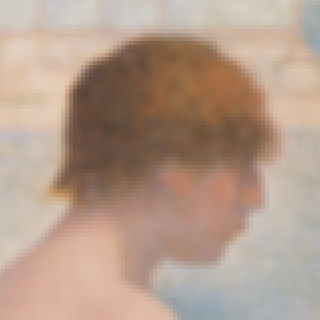
\includegraphics[angle=0,width=0.3\textwidth]{afsnit/vores_implementation/billeder/sloering/simple_3_3}}\hspace{1em}
    \subfloat[$7 \times 7$ vindue]{\label{simple_7_7}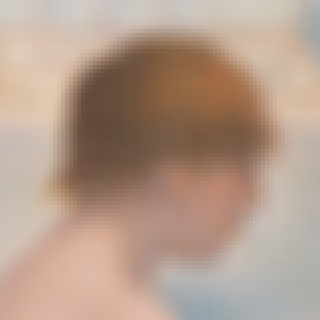
\includegraphics[angle=0,width=0.3\textwidth]{afsnit/vores_implementation/billeder/sloering/simple_7_7}}
    \caption[]{
        \textbf{\ref{simple_original})} Zoom af detajler i det originale billede.
        \textbf{\ref{simple_3_3})}
        \textbf{\ref{simple_7_7})}
    }
    \label{simple_metode}
\end{figure}

\begin{figure}[!h]
    \centering
    \subfloat[Original]{\label{gaussian_original}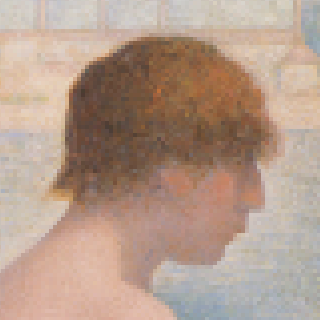
\includegraphics[angle=0,width=0.3\textwidth]{afsnit/vores_implementation/billeder/sloering/original}}\hspace{1em}
    \subfloat[$3 \times 3$ vindue]{\label{gaussian_3_3}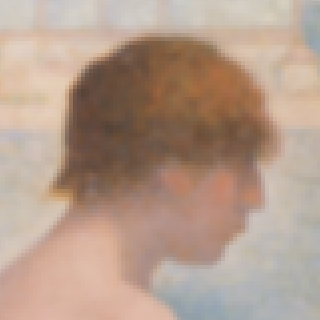
\includegraphics[angle=0,width=0.3\textwidth]{afsnit/vores_implementation/billeder/sloering/gaussian_3_3}}\hspace{1em}
    \subfloat[$7 \times 7$ vindue]{\label{gaussian_7_7}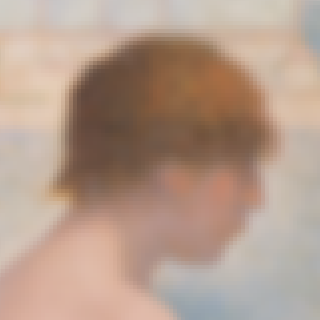
\includegraphics[angle=0,width=0.3\textwidth]{afsnit/vores_implementation/billeder/sloering/gaussian_7_7}}
    \caption[]{
        \textbf{\ref{gaussian_original})} Zoom af detajler i det originale billede.
        \textbf{\ref{gaussian_3_3})}
        \textbf{\ref{gaussian_7_7})}
    }
    \label{gaussian_metode}
\end{figure}

\begin{figure}[!h]
    \centering
    \subfloat[Original]{\label{median_original}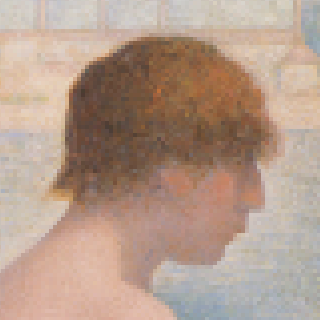
\includegraphics[angle=0,width=0.3\textwidth]{afsnit/vores_implementation/billeder/sloering/original}}\hspace{1em}
    \subfloat[$3 \times 3$ vindue]{\label{median_3_3}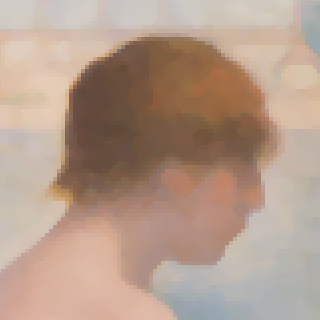
\includegraphics[angle=0,width=0.3\textwidth]{afsnit/vores_implementation/billeder/sloering/median_3_3}}\hspace{1em}
    \subfloat[$7 \times 7$ vindue]{\label{median_7_7}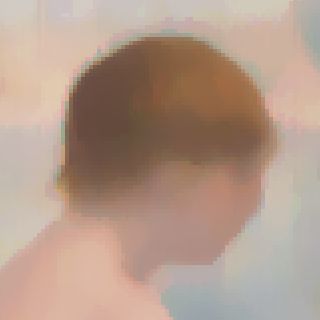
\includegraphics[angle=0,width=0.3\textwidth]{afsnit/vores_implementation/billeder/sloering/median_7_7}}
    \caption[]{
        \textbf{\ref{median_original})} Zoom af detajler i det originale billede.
        \textbf{\ref{median_3_3})} Median med et vindue på $3\times{}3$.
        Farverne er blevet mere ensartede mens kanterne stadig er
        skarpe.
        \textbf{\ref{median_7_7})} Median med et vindue på $7\times{}7$. Farverne
        er meget ensartede, men det ses at kanterne er blevet mere
        udvisket med det større vindue.
    }
    \label{median_metode}
\end{figure}

}

% vim: set tw=72 spell spelllang=da:


\subsection{Kantdetektion}                              % Vi vil gerne afgrænse floodfill
% Denne fil er inkluderet i udtraekning_af_regioner.tex
{
Begrebet kantdetektion dækker over en metode som finder kanterne af
objekter i et billede. Egentlig prøver man at finde de punkter i
billedet, hvor kontrasten er stor, hvilket er tilfældet ved et objekts
grænse. Når vi har fundet kanterne til objekterne i billedet kan vi
bruge disse til at afgøre hvor vi har en ny region i billedet.  Som vi
skal se, så er kantdetektion et godt eksempel på hvor svært datamatsyn
kan være, selv i meget simple algoritmer.

\subsubsection*{Metode}
Der er forskellige algoritmer til rådighed for at finde kanter i
billeder\cite{SIOlsen}. Vi vil beskrive en meget naiv tilgang til
problemet, blot for at forklare grundprincipperne bag metoden. Som
allerede nævnt vil vi finde de steder i billedet hvor vi har stor
kontrast. Det er derfor almindeligt at konvertere billedet til sort/hvid
når man vil finde kanterne. Metoden forklares for én dimension, da det
let kan overføres til to dimensioner. Vi betragter derfor en vektor
$\mathbf{P} = (p_1, p_2, \cdots, p_n)$ som antager værdier i mængden
$\{0,1\}$.

\begin{figure}[!h]
    \renewcommand{\arraystretch}{1.3}
    \centering
    \begin{tabular}{|c|c|c|c|c|c|c|c|c|c|}
        \hline
        1 & 1 & 1 & 1 & 1 & \cellcolor{black}\textcolor{white}{0} & \cellcolor{black}\textcolor{white}{0} & \cellcolor{black}\textcolor{white}{0} & \cellcolor{black}\textcolor{white}{0} & 1\\\hline
    \end{tabular}
    \caption[]{Vektoren $\mathbf{P}$ med tilfældige værdier i mængden
    $\{0,1\}$.}
    \label{vektor_p_edge}
\end{figure}
Vektoren $\mathbf{P}$ kan betragtes som et liniestykke. Vi ønsker nu at
konstruere en ny vektor $\mathbf{E} = (e_1, e_2, \cdots, e_n)$, hvor
$e_i \in \{0,1\}$ ud fra vektoren $\mathbf{P}$. Vi definerer
$\mathbf{E}$ som
\begin{equation}
    \begin{split}
        \mathbf{E} &= (e_1, e_2, \cdots, e_n) \mathrm{~,~hvor~} \\
        &e_i = \left\{
        \begin{array}{rl}
            0 & \text{hvis~} |p_i - p_{i - 1}| = 1\\
            1 & \text{hvis~} |p_i - p_{i - 1}| = 0
        \end{array} \right. \mathrm{,~for~} p_i \mathrm{~i~} \mathbf{P}
        \mathrm{~og~} p_0 = p_1
    \end{split}
    \label{vektor_e_bin}
\end{equation}
Vektoren $\mathbf{E}$ konstrueres altså ved at sammenligne et givet
punkts værdi med det forrige punkts værdi. Hvis den absolutte forskel
til et punkts forgænger er lig $1$ så sættes dette punkt til værdien $0$
i kantvektoren $\mathbf{E}$. Hvis der ikke er nogen forskel sættes værdien til
$1$. Vi er i denne sammenhæng nødt til at definere $p_0$ til $p_1$, så
vi undgår at finde en kant i starten af en linie. Kantvektoren
$\mathbf{E}$ for $\mathbf{P}$ er vist i figur \ref{vektor_e_edge}.

\begin{figure}[!h]
    \renewcommand{\arraystretch}{1.3}
    \centering
    \begin{tabular}{|c|c|c|c|c|c|c|c|c|c|}
        \hline
        1 & 1 & 1 & 1 & 1 & \cellcolor{black}\textcolor{white}{0} & 1 &
        1 & 1 & \cellcolor{black}\textcolor{white}{0} \\\hline
    \end{tabular}
    \caption[]{Kantvektoren $\mathbf{E}$ for $\mathbf{P}$.}
    \label{vektor_e_edge}
\end{figure}
Det ses at $e_6 = e_{10} = 0$, da $|p_6 - p_5| = |p_{10} - p_9| = 1$. Vi
har nu markeret de steder hvor der er kontrast i den oprindelige vektor
$\mathbf{P}$. Vi gør os en vigtig observation vedrørende definitionen på
$\mathbf{E}$. Vi markerer en kant i det punkt hvor kontrasten netop
\emph{er} skiftet. Derfor har vi også at $e_{10}$ bliver markeret som en
kant, selvom man ved manuel inspektion ville markere $e_9$ som kanten.
Dette skyldes at vi ikke har nogen hukommelse i definitionen og derfor
ikke er klar over hvilke punkter der burde hænge sammen. Vi ved altså
ikke hvilke værdier der er de interessante. Denne problematik
understreges af det faktum, at end ikke mennesket altid kan afgøre hvor
grænsen mellem to figurer går. Et klassisk eksempel er den optiske
illusion ved \emph{Rubins vase}\cite{WikiRubinVase} vist i figur
\ref{rubins_vase}. Alt efter hvad man vælger som fokus i billedet, vil
kanten skulle redefineres.

\begin{figure}[!h]
    \begin{center}
        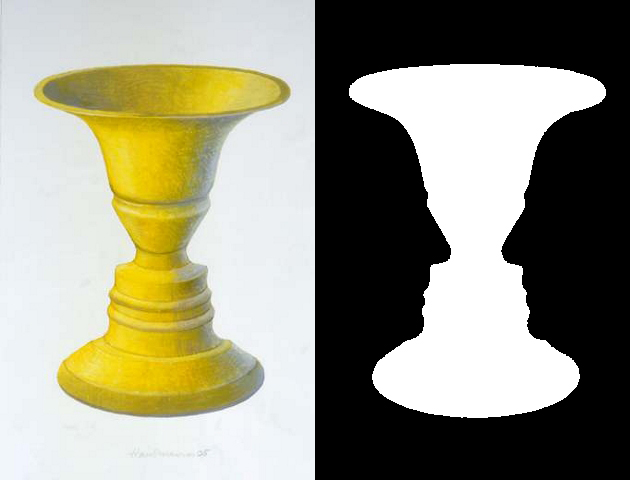
\includegraphics[trim = 84mm 4mm 0mm 0mm, clip, width=3cm]{afsnit/vores_implementation/billeder/kantdetektion/Rubin2}
    \end{center}
    \caption[]{Rubins vase\cite{WikiRubinVasePic}.}
    \label{rubins_vase}
\end{figure}

Vi kan generalisere definitionen for kantvektoren $\mathbf{E}$ i
\ref{vektor_e_bin} således at vi kan have andre værdier end dem i
$\{0,1\}$ og en anden tærskelværdi. I den følgende definition har vi at
$t$ angiver den tærskelværdi, for hvor meget værdierne punkterne imellem
må afvige.
\begin{equation}
    \begin{split}
        \mathbf{E} &= (e_1, e_2, \cdots, e_n) \mathrm{~,~hvor~} \\
        &e_i = \left\{
        \begin{array}{rl}
            0 & \text{hvis~} |p_i - p_{i - 1}| \geq t\\
            1 & \text{hvis~} |p_i - p_{i - 1}| < t
        \end{array} \right. \mathrm{,~for~} p_i \mathrm{~i~} \mathbf{P}
        \mathrm{~og~} p_0 = p_1
    \end{split}
    \label{vektor_e_generel}
\end{equation}

Definitionen på $\mathbf{E}$ tager ikke højde for støj i billedet,
hvilket let kan forvirre kantdetektionen. Sobel kantdetektion er en
etableret metode til at finde kanter i billeder. Den benytter to
foldningsmatricer til at finde kanter vertikalt og horisontalt, men er
ligesom den simple metode følsom overfor støj. Vi benytter os af en
metode udviklet af John F. Canny, da den kombinerer teknikker fra bla.
gaussisk sløring og Sobel\cite{SIOlsen}, og således ikke ligeså følsom overfor
støj. Vi vil ikke komme nærmere ind på den indre funktionalitet i Canny,
men vi vil i det følgende vise eksempler på resultater fra metoden.

\subsubsection*{Eksempler}
Vi viser nu nogle eksempler på hvordan Canny kantdetektion virker. Vi
tager igen udgangspunkt i maleriet i figur \ref{bathers}. Billedet
bliver først konverteret til gråtoner som da bruges til at finde kanter
i. Metoden returnerer et nyt sort billede med hvide kanter. Billederne
der vises er således ikke det direkte resultat fra metoden, men vi viser
kun de dele af originalbilledet hvor metoden har fundet kanter. Metoden
bruger to tærskelværdier som kan justeres alt efter hvor mange detajler
man ønsker. Vi vil ved hjælp af de følgende eksempler komme frem til
hvad tærskelværdierne betyder for resultatet. Eksemplerne er samlet i
figur \ref{canny_kanter}.

\begin{figure}[!p]
    \centering
    \subfloat[$(20, 20)$]{
        \label{canny_20_20}
        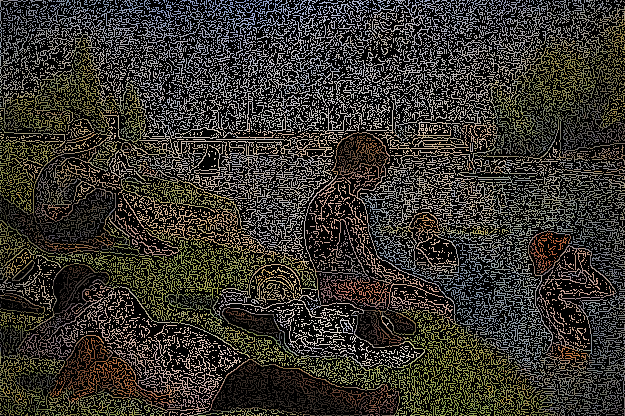
\includegraphics[width=0.6\textwidth]{afsnit/vores_implementation/billeder/kantdetektion/canny_20_20}}\\
    \subfloat[$(20, 100)$]{
        \label{canny_20_100}
        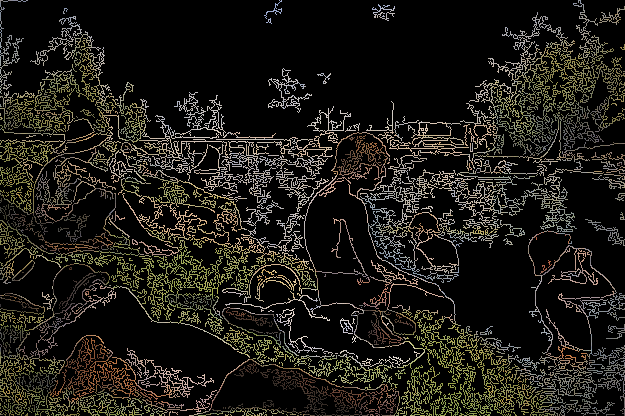
\includegraphics[angle=0,width=0.45\textwidth]{afsnit/vores_implementation/billeder/kantdetektion/canny_20_100}}\hspace{1em}
    \subfloat[$(60, 150)$]{
        \label{canny_60_150}
        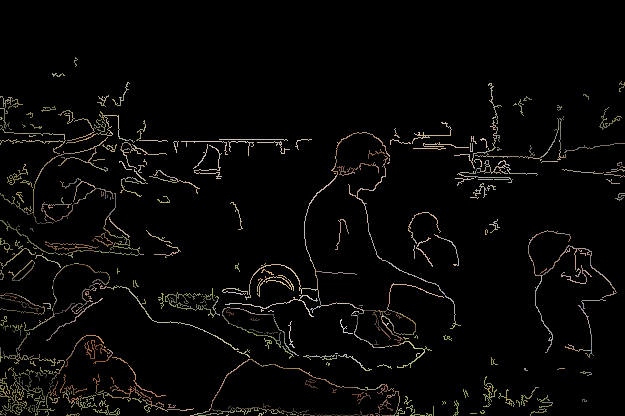
\includegraphics[angle=0,width=0.45\textwidth]{afsnit/vores_implementation/billeder/kantdetektion/canny_60_150}}\\
    \subfloat[$(70, 175)$]{
        \label{canny_70_175}
        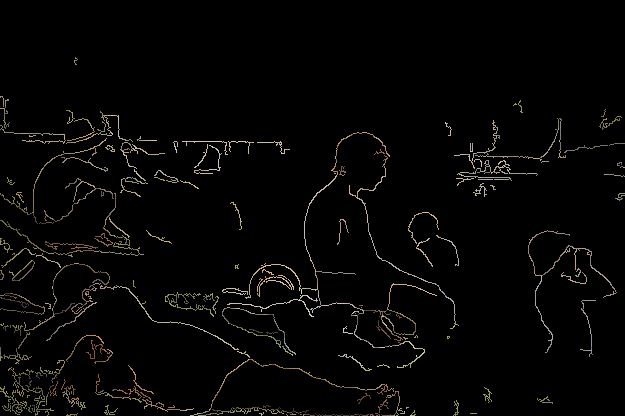
\includegraphics[angle=0,width=0.45\textwidth]{afsnit/vores_implementation/billeder/kantdetektion/canny_70_175}}\\
    \subfloat[$(100, 295)$]{
        \label{canny_100_290}
        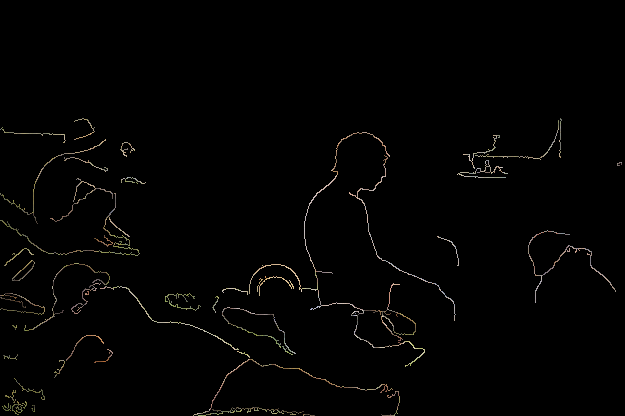
\includegraphics[angle=0,width=0.6\textwidth]{afsnit/vores_implementation/billeder/kantdetektion/canny_100_290}}
    \caption[]{Forskellige resultater med Canny kantdetektion.
    Tærskelværdierne er noteret under billederne.}
    \label{canny_kanter}
\end{figure}

Når vi sammenligner figur \ref{canny_20_20} og \ref{canny_20_100} ses
det at anden parameter lader til at ignorere kanter som ligger ``inden
for'' andre kanter. Dette ses på stort set alle personernes kroppe i
billedet. Når denne observation er gjort, prøver vi at skrue op for
tærskelværdierne. Det ses at ved højere tærskelværdier bliver billedet
med kanter gradvist mindre detaljeret. I vores testbillede er kanterne
på de fremtrædende objekter stadig at se, selv ved store tærskelværdier
som vist i \ref{canny_100_290}. Vi vil i kapitel \ref{chap_afproevning}
se på hvilke tærskelværdier vi bruger i praksis.
}

% vim: set tw=72 spell spelllang=da:


\subsection{Sammensætning af metoder}
Forklar hvordan vi kombinerer metoderne

}

% vim: set tw=72 spell spelllang=da:
